\chapter{Planificación temporal}\label{cap:9}
Normalmente, los proyectos de ingeniería tienen establecidos unos objetivos principales o metas definidas al inicio del mismo, esto es, la finalidad perseguida queda claramente determinada y deben alcanzarse dichos objetivos durante el tiempo marcado al comienzo, cumpliendo las exigencias requeridas y utilizando los recursos puestos a disposición de las personas encargadas de llevar a cabo el proyecto. La planificación temporal, se realiza durante las primeras fases y consiste esencialmente en realizar la \emph{\acrfull{edp}} o \emph{\acrfull{wbs}} y, posteriormente, el conocido \emph{Diagrama de Gantt}.

De esta manera, el trabajo puede dividirse en bloques o paquetes \enquote{entregables} con un orden lógico, estableciendo el alcance para, después, completar la duración de las actividades asociadas y sus relaciones de precedencia que aparecen explícitamente representadas mediante el Diagrama de Gantt mencionado. En el ámbito de la investigación, en general, no es habitual presentar esta organización sistemáticamente, aunque la concesión de proyectos de investigación necesita proponer unos objetivos y tiempos para obtener la financiación necesaria. 

En este Trabajo Fin de Máster, la división del trabajo está formada por cuatro grupos con sus actividades entregables correspondientes, como muestra la Figura \ref{fig:ch9_edp}. El primer grupo está formado por las tareas iniciales de documentación y recopilación de los artículos, junto al proceso de aprendizaje del código Dagon utilizado durante las simulaciones; el segundo grupo, constituye el estudio de la información obtenida y el lanzamiento de las primeras simulaciones y pruebas; el tercer grupo, dedicado a la organización y estructura de las distintas partes del trabajo, así como continuar con el proceso de ejecución de las simulaciones; y, finalmente, el último grupo donde terminan las simulaciones y comienza el proceso de redacción y maquetación de la memoria.

\begin{figure}[htbp]
  \centering
  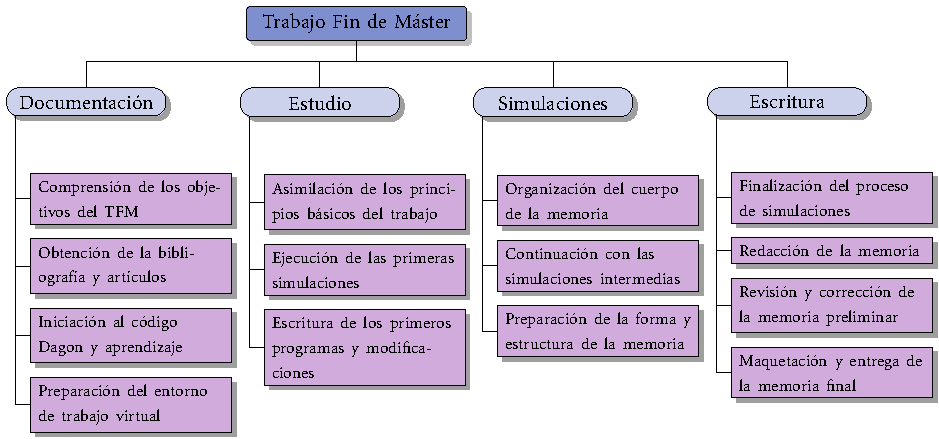
\includegraphics[width=\textwidth]{Figuras/ch9_edp.pdf}
  \caption{Estructura de Descomposición del Proyecto.}
  \label{fig:ch9_edp}
\end{figure}

Establecido el alcance temporal y las actividades necesarias, queda determinar las relaciones entre estas actividades y sus tiempos de duración. La duración total del proyecto, mostrada gráficamente en la Figura \ref{fig:ch9_gantt}, se extiende desde aproximadamente el $3$ de octubre de $2022$ hasta la última quincena de enero de $2024$, es decir, tres cuatrimestres consecutivos entre los cursos académicos \numrange{2022}{2023} y \numrange{2023}{2024}. El diagrama proporciona algunos hitos importantes, así como las relaciones de precedencia mencionadas entre los distintos bloques.

Un primer vistazo al diagrama demuestra que la planificación temporal presenta una distribución lineal de los distintos entregables, es decir, desde el comienzo del trabajo estaba previsto seguir una secuencia donde unas actividades terminan y, inmediatamente después, comienzan las siguientes actividades sucesoras. Las simulaciones realizadas emplean este algoritmo lineal, pues los métodos numéricos requieren un tiempo de ejecución prolongado y, principalmente, debido a la necesidad de hacer un estudio previo de las imágenes extraídas para determinar los siguientes grupos de simulaciones a realizar y los parámetros utilizados. Por este motivo, los bloques dedicados a analizar los resultados están repartidos a lo largo de la duración total del proyecto. 

\begin{figure}[htbp]
  \centering
  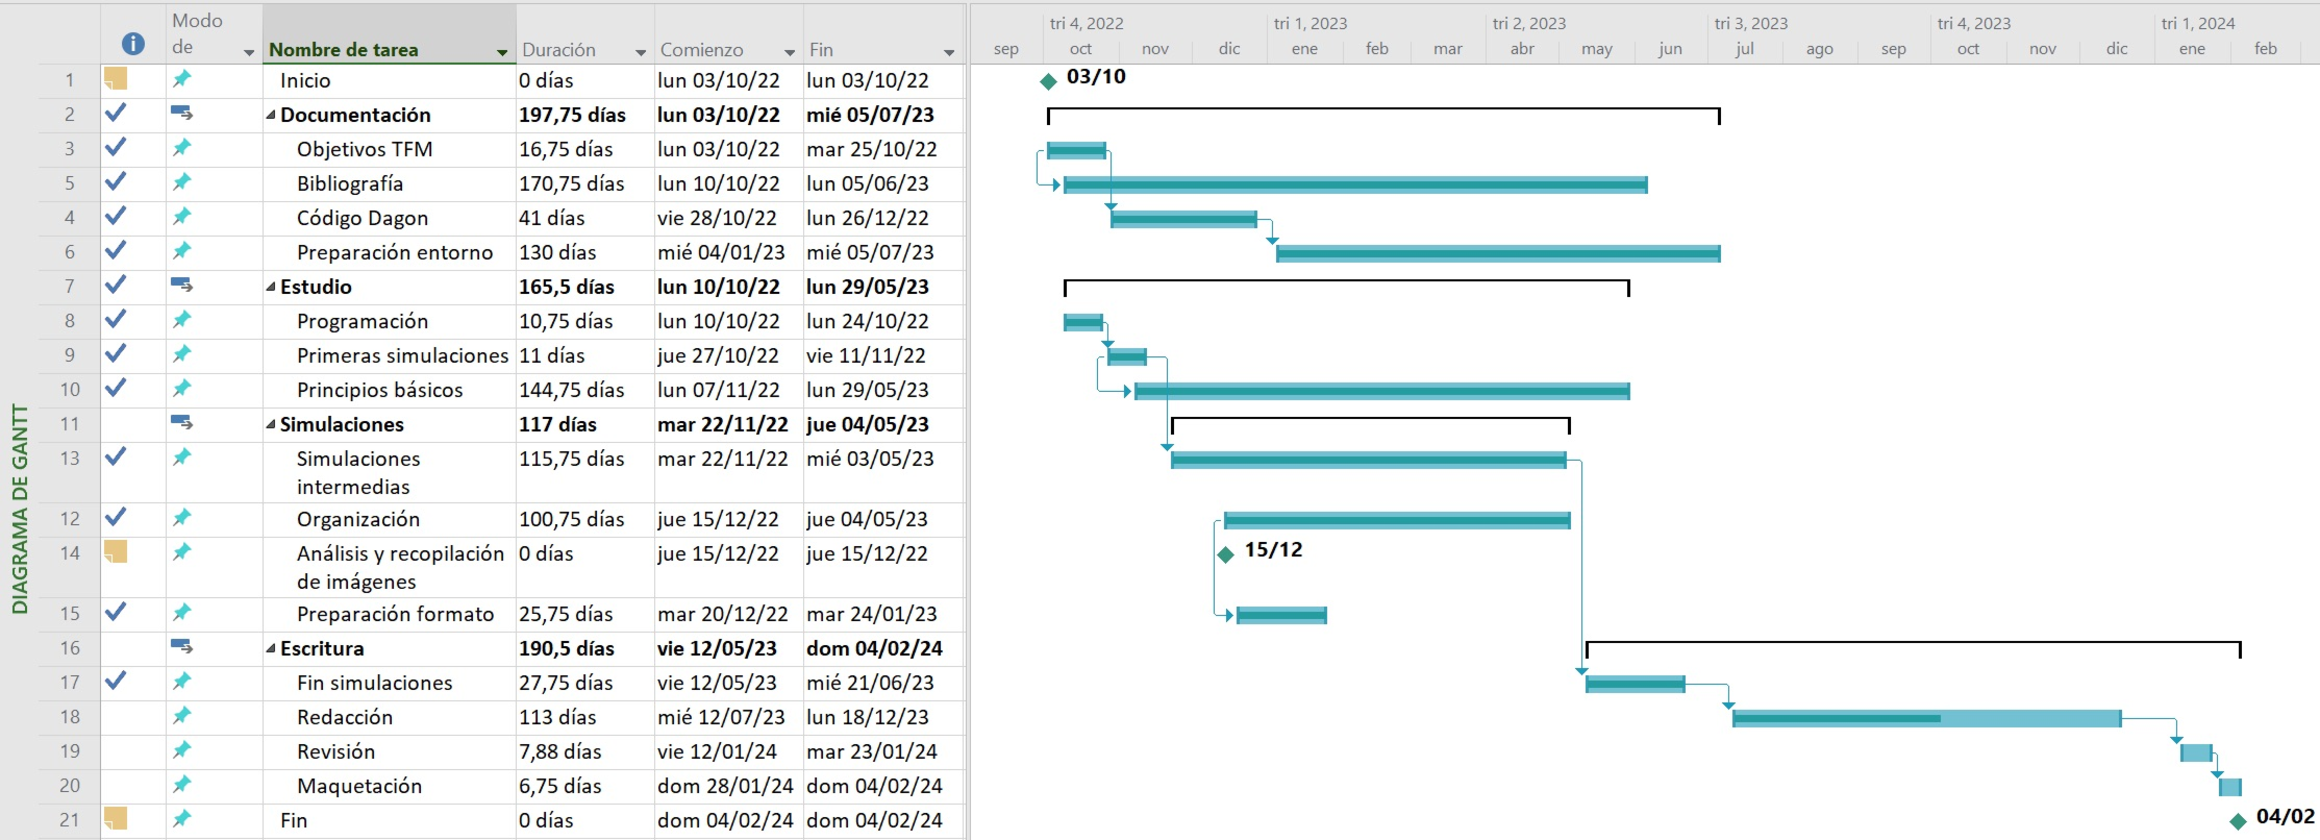
\includegraphics[height=7.5cm,width=\textwidth]{Figuras/ch9_gantt.pdf}
  \caption{Diagrama de Gantt del proyecto}
  \label{fig:ch9_gantt}
\end{figure}


